\chapter{Kinemato-static model}
A kinematostatic model is a model that combines kinematics (motion and geometry) with statics (forces and equilibrium) to describe how a mechanical system moves and how forces are transmitted through it.

\section{Kinematic model}

\begin{figure}
    \centering
    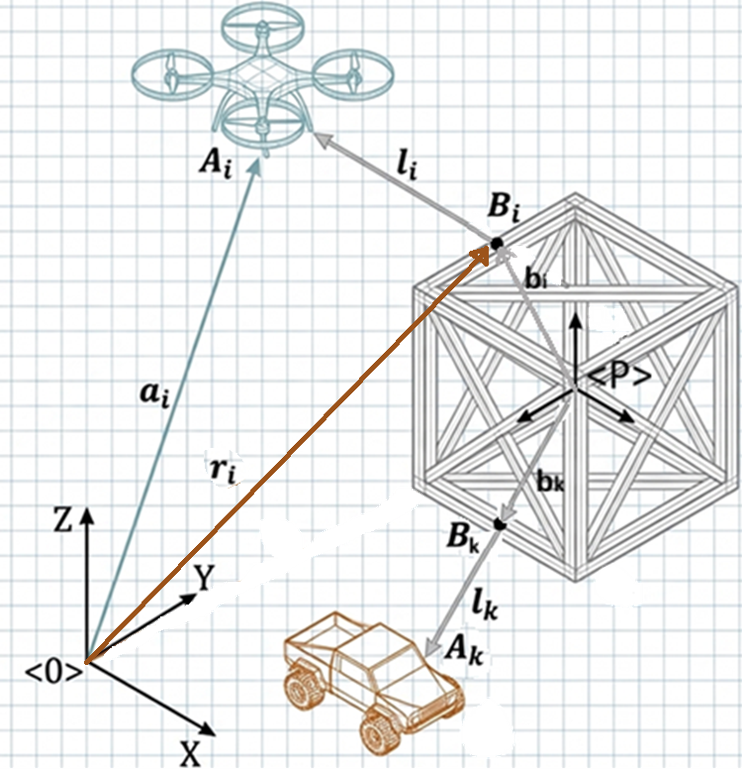
\includegraphics[width=0.5\linewidth]{images/platform_framework.png}
    \caption{Graphical representation of the platform}
    \label{fig:platform_connection_graphical_representation}
\end{figure}

Given the payload twist $^0\xi = \begin{bmatrix}
    ^0v_p & ^0\omega_p
\end{bmatrix}^\top$ in the inertial reference frame $<0>$, we can write the position and velocity of the attachment point $B_i$ (resp. $B_k$) of the aerial vehicle (resp. ground) in $<0>$.
\begin{equation}
    ^0\boldsymbol{r}_i = ^0\boldsymbol{p} + \, ^0_PR \, ^P\boldsymbol{b}_i
\end{equation}
where $b_i$ is the attachment point on payload.
\begin{equation}
    ^0\dot{\boldsymbol{r}}_i = ^0\boldsymbol{v}_p + ^0\boldsymbol{\omega}_p \times \left( ^0_PR \, ^P\boldsymbol{b}_i \right)
    \label{eq:attachmentpointvelWRTinertialframe}
\end{equation}

For definition, the cable vector is $\boldsymbol{l}_i = \boldsymbol{a}_i - \boldsymbol{r}_i = A_i - B_i$ with $\boldsymbol{a}_i$ being the anchor position. 
Under a centralized controller, the positions of all UAV $A_i$ and UGV $A_k$ are known, which directly determin the anchor vector $\boldsymbol{a}_i$. Furthermore, he payload's position and orientation are assumed to be known.ogether with the known locations of the attachment points relative to the payload, this information allows us to calculate the cable vectors $\boldsymbol{l}_i$.

The final form of cable vector variation is given by applying Equation \ref{eq:attachmentpointvelWRTinertialframe} in its definition:

\begin{equation}
    \dot{\boldsymbol{l}}_i = \dot{\boldsymbol{a}}_i - \dot{\boldsymbol{r}}_i = \dot{\boldsymbol{a}}_i - \frac{d}{dt}\left(\boldsymbol{p} + \, _PR \, ^P\boldsymbol{b}_i \right) =\dot{\boldsymbol{a}}_i - \left(\boldsymbol{v}_p + \boldsymbol{\omega}_p \times \left( _PR \, ^P\boldsymbol{b}_i \right)\right)
\end{equation}


Each $\dot{l}_i$ corresponds to the projection of the relative velocity of $B_i$ along the cable direction
\begin{equation}
\begin{aligned}
    \dot{l}_i 
    &= u_i^\top \left( 
        \dot{\boldsymbol{a}}_i 
        - \left( 
            \boldsymbol{v}_p 
            + \boldsymbol{\omega}_p \times (\, _P R \, ^P\boldsymbol{b}_i ) 
        \right) 
    \right) \\
    &= u_i^\top \dot{\boldsymbol{a}}_i 
    - 
    \begin{bmatrix}
        u_i^\top & (\, _P R \, ^P b_i \times u_i )^\top
    \end{bmatrix}
    \xi \\
    &= J_{a,i}\, \dot{a}_i - J_{p,i}\, \xi ,
\end{aligned}
\label{eq:cablelengthrate}
\end{equation}
This gives us the kinematic model that relates the variation of cable length vector $\boldsymbol{\rho}$ with the change in position of the anchors and the payload twist:
\begin{equation}
    \dot{\rho} = J_a \dot{a} - J_p \xi = J_a \begin{bmatrix}
        \dot{a}^{(a)} \\ \dot{a}^{(g)}
    \end{bmatrix} - J_p \xi
    \label{eq:kinematic_model}
\end{equation}

Let $m = n_a + n_g$ be the total number of winches (or cables) and $u_i = l_i/\|l_i\|$ the unit cable direction , then:
\begin{itemize}
    \item $\dot{\rho} = \begin{bmatrix}
        \dot{l}_1 & \dot{l}_2 & \dots & \dot{l}_m
    \end{bmatrix}^\top$ is the cable length rate (dimension $[m\times1]$). 

    \item $J_a$ is the Jacobian relating the anchor velocities to the cable-length rates $[m\times3m]$. In particular, each cable depends only on its anchor velocity.
    
\begin{equation}
J_a =
\begin{bmatrix}
u_1 & 0   & \cdots & 0 \\
0   & u_2 & \cdots & 0 \\
\vdots & \vdots & \ddots & \vdots \\
0 & 0 & \cdots & u_{n_a + n_g} \\
\end{bmatrix},
\qquad
u_j = \frac{(a_j - r_j)}{\|a_j - r_j\|}.
\label{eq:cableVector}
\end{equation}
    \item $J_p$ is the Jacobian relating the payload twist to the cable-length  $[m\times6]$
\end{itemize}
\begin{equation}
    J_p =
\begin{bmatrix}
u_1^\top & \left( \, _pR\, ^pb_1 \times u_1 \right)^\top \\ 
\vdots & \vdots \\
u_m^\top & \left( \, _pR\, ^pb_m \times u_m \right)^\top \\
\end{bmatrix}
\end{equation}
\begin{note}
    Equation \ref{eq:cablelengthrate} contains $m$ equations in 6 unkown. I need at least six independent cable directions ($\text{rank}(J_p) = 6$).
\end{note}

\noindent The control allocation matrix maps the actuator inputs (cable tension vector) to the system (payload) wrench. For this definition $J_p^\top$ is the allocation matrix.
\begin{equation}
    W_p = J_p^\top \tau
\end{equation}
Let $W_p^*$ being the desired payload wrench, the control allocation problem to solve is
\begin{equation}
    J_p^\top \tau = W_p^*, \qquad \text{s.t}. \tau_i > 0
\end{equation}

\section{Static model}
Let $\tau=[\tau_{uav}^\top, \tau_{ugv}^\top]^\top\in \mathbb{R}^{m\times 1}$ the cable tension vector, then
\begin{equation} 
\begin{aligned}
    \underbrace{\tau^\top\dot{\rho}}_{\text{total cable power}} &= \underbrace{\tau^\top J_a\dot{a}}_{\text{UAVs and UGVs mechanical power}} - \underbrace{\tau^\top J_p \, \xi}_{\text{payload power}} \\
    &= (J_a^\top \tau)^\top \dot{a} - (J_p^\top \tau)^\top \xi\\
    &= F_a^\top \, \dot{a} - W_p^\top \, \xi
\end{aligned}
\end{equation}

Each cable $i$ applies a force on the payload $F_{a, i}$ and an equal and opposite force on the UAV (resp. UGV). We can write balance equation on our elements:

\subsubsection{Payload Balance}
\begin{equation}
    \underbrace{W_p}_ {J_p^\top \tau } + \underbrace{W_g}_{\begin{bmatrix}
        0 \\0 \\ - m_p g \\ 0\\ 0\\ 0\\
    \end{bmatrix}} + W_{contact}
 + \underbrace{W_{wind}}_{\parbox{2cm}{\centering let = 0}} = 0
 \label{eq:payloadbalance}
\end{equation}
where since each cable produces a wrench on the payload, the contribution given by the $i$-th cable is:
\begin{equation}
    \underbrace{w_{p,i}}_{6\times 1} = \underbrace{J_{p,i}^\top}_{6\times1} \, \underbrace{\tau_i}_{1\times 1}  = \begin{bmatrix}
        u_i^\top & (\, _P R \, ^P b_i \times u_i )^\top
    \end{bmatrix}^\top \tau_i = \begin{bmatrix}
        \tau_i u_i \\ (\, _P R \, ^P b_i \times \tau_i u_i )
    \end{bmatrix}
\end{equation}
and $W_{contact} = 0$ when there is no contact with the environment.

\subsubsection{UAV balance} % at the attachment point $A_i$
\begin{equation}
    -F_{a,i} + F_{prop, i} + \underbrace{F_{g,i}}_{\begin{bmatrix}
        0 \\ 0 \\ - m_{i} g
    \end{bmatrix}} = 0
    \label{eq:uavbalance}
\end{equation}
with $^iF_{prop} = \begin{bmatrix}
        0 & 0 & F_{prop,z,i}
    \end{bmatrix}^\top$ and $F_{a, i} = J_{a, i}^\top \tau_i = \tau_i u_i$.

UAVs must always generate sufficient thrust to maintain flight and ensure their own stability. As a result, only a portion of their available thrust can be allocated to payload manipulation, which reduces the effective force that can be transmitted through the cables.

\subsubsection{UGV balance}
\begin{equation}
    -F_{a,j} + \underbrace{F_{ground, j}}_{\begin{bmatrix}
        F_{frict,x,j} \\ F_{frict,y,j} \\ F_{norm}
    \end{bmatrix}} + \underbrace{F_{g,j}}_{\begin{bmatrix}
        0 \\ 0 \\ - m_{j} g
    \end{bmatrix}} = 0
    \label{eq:ugvbalance}
\end{equation}
with $\|F_{frict}\| \le \mu F_{norm}$ and $F_{norm} = m_j g - F_{a, z, j}$ and $F_{a,j}$ is obtained through Equation \ref{eq:Fai}.

Similarly, UGVs are subject to ground interaction constraints. In particular, they must satisfy friction limits to remain stationary when no motion is commanded. This imposes bounds on the admissible cable forces, as excessive tension may cause slipping.


\noindent By Newton's third law, the force the cable exerts on the drone $F_{a, i}$ (resp. on the UGV $F_{a, j}$) is equal and opposite to the force it exerts on the payload. Since $u_i$ points from $B_i$ toward $A_i$, the cable pulls the drone with
\begin{equation}
    F_{a, i} = J_{a, i}^\top \tau_i = \tau_i u_i
    \label{eq:Fai}
\end{equation}
As a consequence, the total cable force on the payload is:
    \begin{equation}
        F_p = -\sum_{i=1}^{n_a} F_{a, i} -\sum_{j=n_a + 1}^{n_a + n_g} F_{a, j}
        \label{eq:ForceOnPayload}
        \end{equation}
where the payload wrench is $W_p = \begin{bmatrix}
    F_p & M_P
\end{bmatrix}^\top$

\begin{figure}
    \centering
    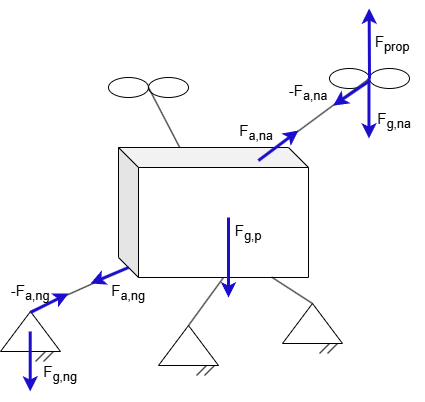
\includegraphics[width=0.5\linewidth]{images/force_on_system.png}
    \caption{Forces acting on the ACTS}
    \label{fig:forceonACTS}
\end{figure}

\section{Kinemato-static model}
Writing Equation \ref{eq:payloadbalance}, \ref{eq:uavbalance} and \ref{eq:ugvbalance} in term of $\tau$, we obtain:
\begin{equation}
    W_{sys} = \begin{bmatrix}
        W_p \\ F_a
    \end{bmatrix} = 
    \begin{bmatrix}
        J_p^\top \\ J_a^\top
    \end{bmatrix} \tau = G\tau = \begin{bmatrix}
        -W_g - W_{contact} - W_{wind} \\
        F_{prop} + F_{ground} + F_g
    \end{bmatrix}
\end{equation}
where $F_{prop,j} = 0$ for the UGVs and $F_{ground, i} = 0$ for the UAVs. Then $W_{sys}$ is $(6+3m)\times 1$ and
\begin{equation}
    G\tau + \begin{bmatrix}
        W_g + W_{contact} + W_{wind} \\
        - F_{prop} - F_{ground} - F_g
    \end{bmatrix} = 0
\end{equation}

